\chapter{Dataset}
\label{ch:dataset}

% Overall goals of chapter

% Explain what configuration/data is desired for the analysis.
% Explain that Science Park stations are going to be the focus.
% It is best suited because of high density of stations, and known configurations.
% Show what data is available to work with.
% Show that much of the data remains after cuts and will be used in the next chapter.


\section{What the dataset will be used for}

% Direction reconstructions requires 3 or more stations (or detectors)
% Preferably triangular shape, at least not to much on a line.
% Stations must be close enough together (\SI{<1}{\kilo\meter}) to have lot of detections for statistics.
% Uptime must be good, specifically simultaneous uptime of stations.
% Properly configured station to make triggering similar.


\section{Choice of cluster}

% Possible clusters with close stations: Zaanlands/SciencePark/Twente/Eindhoven.
% Science Park for main analysis, because it has most potential for exploring the shower front. Highest sampling for each shower.
% All stations have 4 detectors and are capable of stand-alone reconstruction.
% Science park stations have good uptime.
% Mean/noise filter disabled for long period for good trigger time reconstruction.
% Large distance between outer detectors, detectors in between useful for accurate station timing offsets and more accurate reconstructions.

\begin{figure}
    \centering
    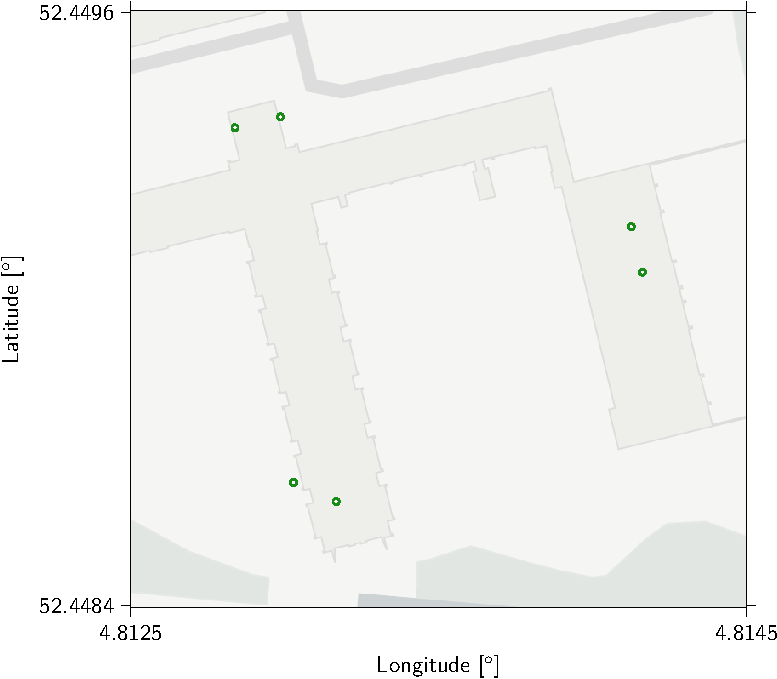
\includegraphics[width=0.23\linewidth]{plots/dataset/stations_102_104_105_detectors.pdf}
    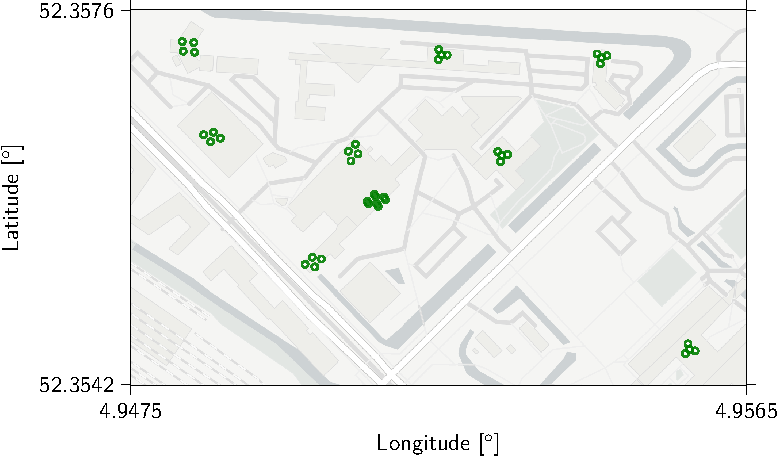
\includegraphics[width=0.23\linewidth]{plots/dataset/stations_501_502_503_504_505_506_508_509_510_511_detectors.pdf}
    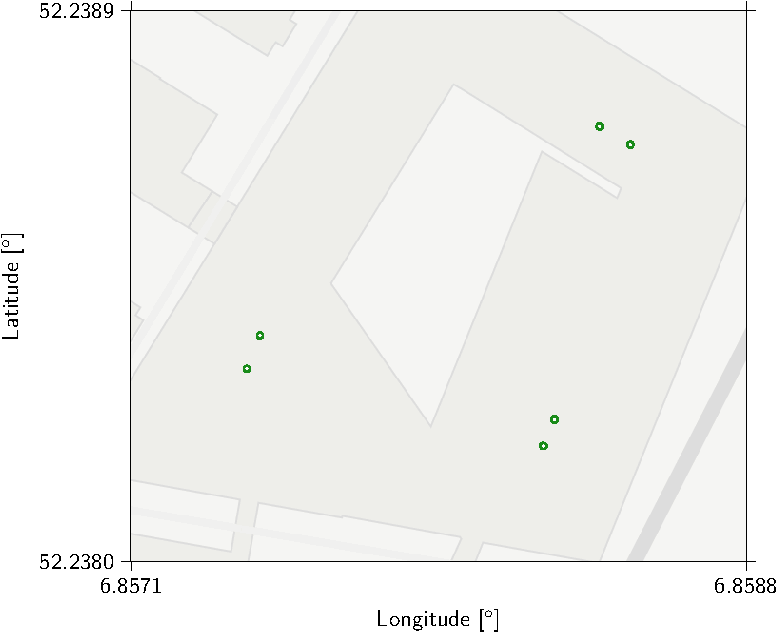
\includegraphics[width=0.23\linewidth]{plots/dataset/subcluster_7000.pdf}
    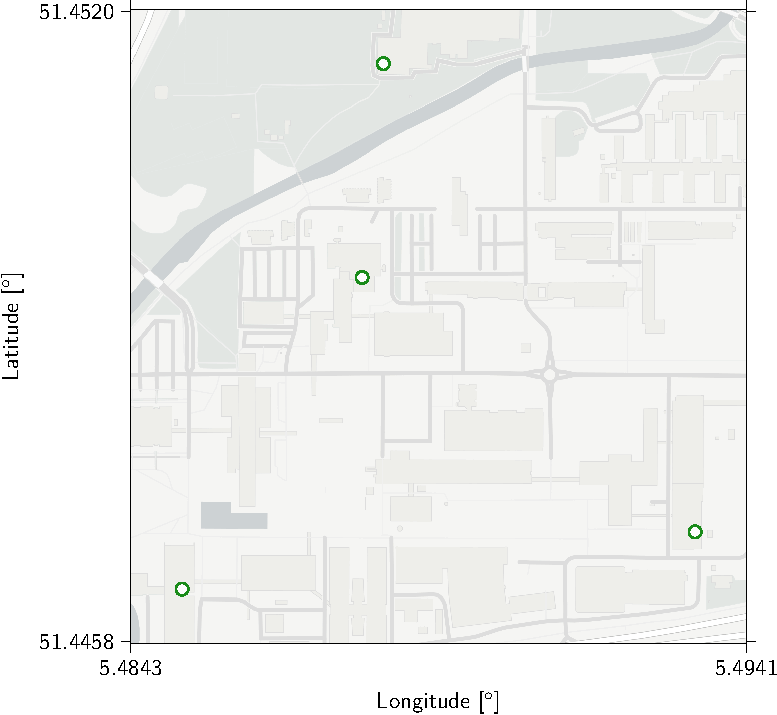
\includegraphics[width=0.23\linewidth]{plots/dataset/stations_8001_8004_8008_8009.pdf}
    \caption{Several compact station clusters. All present excellent opportunities for reconstructions of showers. However, the Science Park cluster is the only with many 4-detector stations.}
    \label{fig:compact_clusters}
\end{figure}



\section{Raw data}

% Start date for each station and number of raw triggered events

Table to show start dates of each station

\begin{verbatim}
    Start        Station  N
    2004-03-26   501      220e6
    2008-08-02   502      120e6
    2008-08-02   503      130e6
    2008-08-02   504      150e6
    2008-08-07   505      120e6
    2008-08-03   506       80e6
    2013-06-17   508       30e6
    2005-01-31   509      120e6
    2014-09-29   510       30e6
    2015-06-16   511       10e6
\end{verbatim}

\section{Data cuts}

% Cut based on date to use data after 2011-6 to ensure GPS time is used, instead of UTC time.
% Cut days on which configuration changed.
% Cut station or detector for entire day or single event, show examples of cuts for various parameters.
% If detector is working badly, better to exclude for entire day, and ignore it for particle density.
% Check that bad data does not introduce unwanted bias.

Exclude days on which configuration of a station is changed, part of the day will have different configuration, and sometimes config is sent to late, or quickly changed again. (Approximate values used in tables.)

\begin{verbatim}
    changed param   501 502 503 504 505 506 508 509 510 511
    GPS             23  8   7   4   11  3   1   4   10  1
    electronics     3   3   1   1   2   3   2   1   0   0
    PMT voltages    21  16  23  17  23  12  6   6   8   2
    Total days      [number of unique days to be excluded]
\end{verbatim}

\begin{figure}
    \centering
    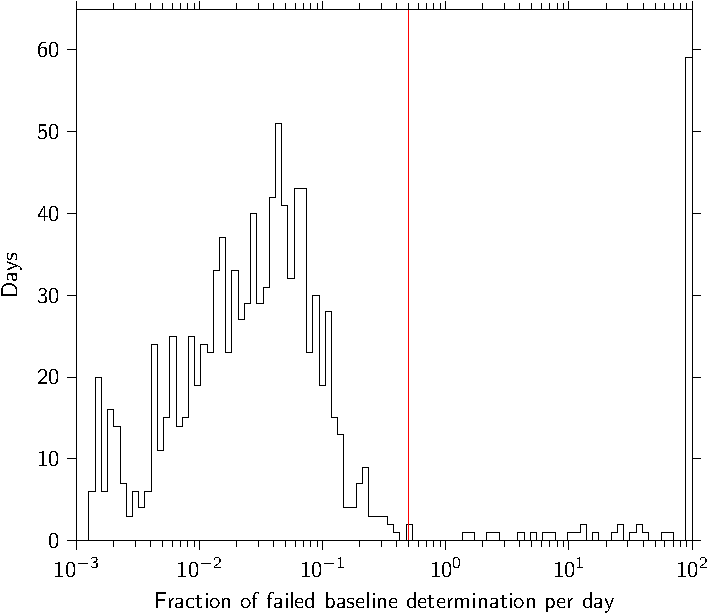
\includegraphics[width=0.7\linewidth]{plots/dataset/histogram_failed_baseline_504_4.pdf}
    \caption{Histogram of fraction of failed baseline determinations per day for a detector for station 504. Up to \SI{0.5}{\percent} appears normal, higher indicates problem with the detector and it may be best to exclude it for the entire day.}
    \label{fig:bad_baseline}
\end{figure}

Remaining number of events per station after cuts.

\begin{verbatim}
    Station  N after cut
    501      97e6
    502      66e6
    503      71e6
    504      86e6
    505      70e6
    506      76e6
    508      32e6
    509      82e6
    510      24e6
    511       8e6
\end{verbatim}

The number of coincidences before and after the cuts with at least n stations in coincidence. Number of coincidences with at least 2 stations in coincidence: 13391318.

\begin{verbatim}
    N   Before cut   After cut
    3   1975275      ....
    4   544342       ....
    5   187480       ....
    6   71286        ....
    7   27552        ....
    8   9714         ....
    9   3111         ....
    10  787          ....
\end{verbatim}

\begin{figure}
    \centering
    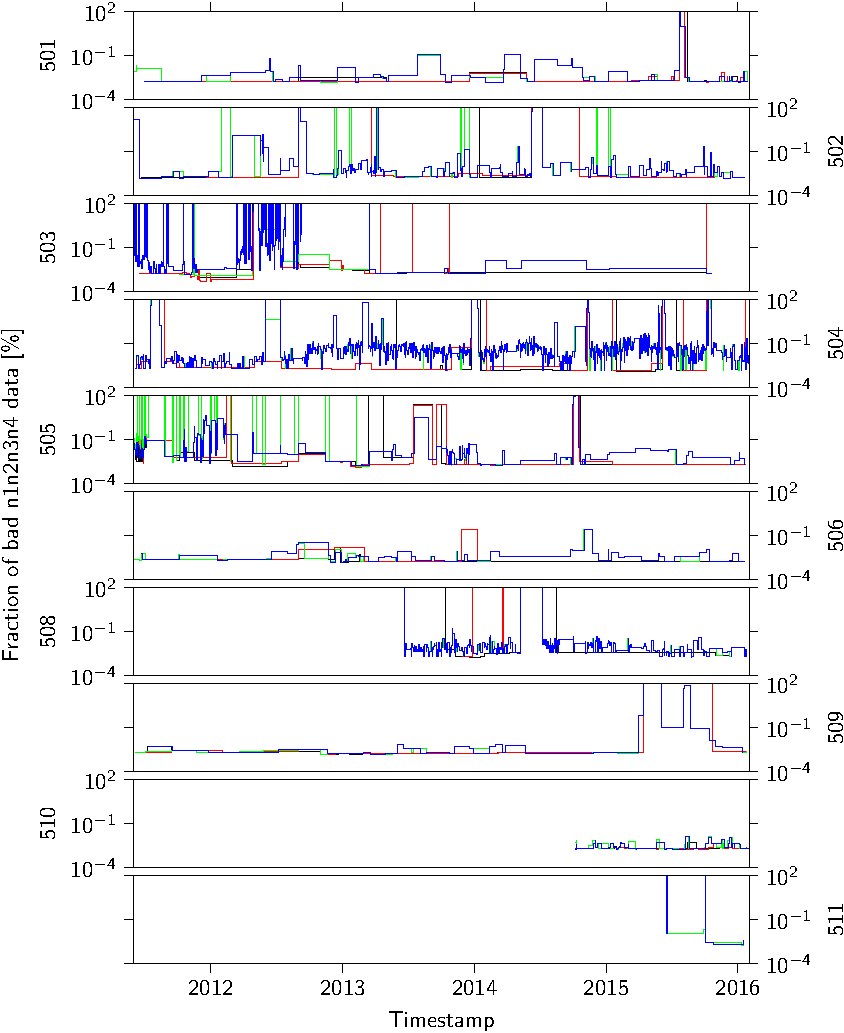
\includegraphics[width=0.7\linewidth]{plots/dataset/bad_fraction_n1n2n3n4.pdf}
    \caption{If bad fraction is higher than \SI{.5}{\percent} discard the detector for entire day. If below, exclude only that detector for those events.}
    \label{fig:bad_n}
\end{figure}
